\begin{figure}[H]\caption{•}\label{fig:equilibrium}
\center
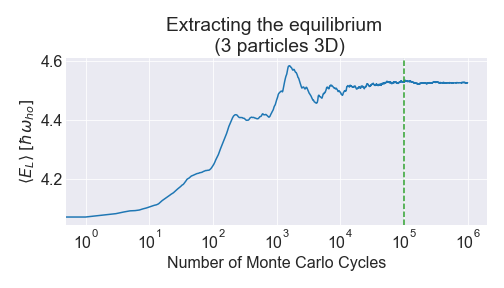
\includegraphics[width=0.7\linewidth]{../Results/equilibrium}
\end{figure} 
 
 \subsection{Analytical versus numerical evaluation of the double derivative}
 
\begin{table}[H]\caption{A comparison of the CPU time of calculating the double derivative analytically and numerically. Here N is the number of particles and these calculations were performed in three dimensions. The numbers in the table are an average of 10 runs.}
\center
\begin{tabular}{l|ll|l}
& CPU time [s]&\\
N & Analytical & Numerical & Ratio $\nicefrac{num}{ana}$\\ \hline
1 & 1.6319 & 2.7882 & 1.7085\\
2 & 2.3090 & 8.2743 & 3.5835\\
4 & 3.5503 & 14.5833 & 4.1076\\
6 & 4.7517 & 29.1024 & 6.1246\\
8 & 6.0642 & 48.4739 & 7.9934\\
10 & 7.6771 & 67.4531 & 8.7863\\
\end{tabular}
\end{table}

\subsection{No interaction - brute force sampling}

\subsubsection{Comparison with exact values}

Figure \ref{fig:exact_comparison_1D} shows the energies of the Bose gas. These calculations were performed with brute force sampling and the particles are not interacting with each other. The exact energy for $N$ number of particles in $d$ dimensions is given by

\begin{equation}\label{eq:exact_energy_expression}
\left< E \right> =\left( \frac{1}{2}\alpha + \frac{1}{8 \alpha}\right)Nd
\end{equation}

which was found from the one particle in one dimension case in Ref. \cite{GriffithsDavidJ1995Itqm}. Equation \ref{eq:exact_energy_expression} is in natural units where $m = 1$, $\hbar = 1$ and $\omega = 1$. The parameter that gives the minimum of the exact energy is easily found from the derivative of Eq. \ref{eq:exact_energy_expression} with respect to $\alpha$
$$ \frac{d \left<E\right>}{d \alpha}  = \left(\frac{1}{2} - \frac{1}{8\alpha^2}\right)Nd = 0 \implies \alpha = \frac{1}{2}. $$
The energy when $\alpha = 0.5$ is then
$$ \left< E(\alpha = 0.5)\right> = \left(\frac{1}{4} + \frac{2}{8}\right)Nd = \frac{1}{2}Nd $$
We see that this is the case in Fig. \ref{fig:exact_comparison_1D}, where all the energies follow the exact curve since the energy is plotted in energy per particle and all calculation are done in one dimension. We observe some variations from the exact values, but the calculation were done with only $2^{19} \approx 5.2\cdot10^{5}$ MC cycles. 

\begin{figure}[H]
\center
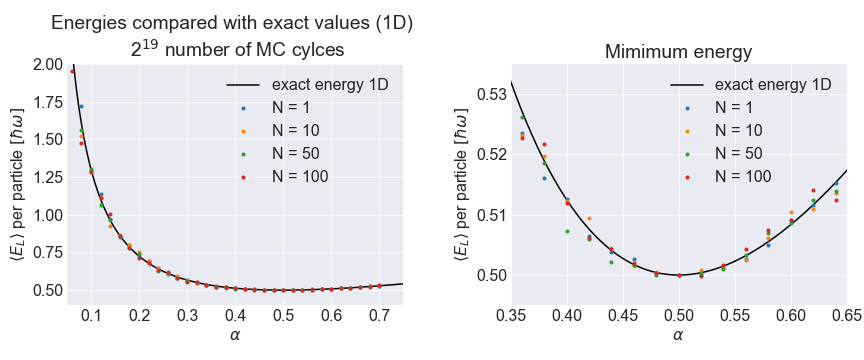
\includegraphics[width=\linewidth]{../Results/comparing_with_exact_1D}\caption{Energy of the boson gas for a range of different parameters $\alpha$. Here $N$ is the number of particles. And the exact energy is calculated using Eq. \ref{eq:exact_energy_expression}. Left: The exact energy for one particle in one dimension including the calculated energies per particle, so they can be easily compared. Right: A closer look at the minimum point of the curve.}\label{fig:exact_comparison_1D}
\end{figure}

\begin{table}[H]\caption{Exact expectation values for the systems relevant in this project. Here $d$ is the number of dimensions and $N$ is the number of particles. The energies are of units $\hbar \omega_{ho}$.}\label{tab:exact_values}
\center
\begin{tabular}{rrr|rrr|rrr}
$d$ & $N$ & $\left< E_L \right>$ &$d$ & $N$ & $\left< E_L \right>$&$d$ & $N$ & $\left< E_L \right>$\\ \hline
&1 & 0.5 &&1 & 1.0 &&1 & 1.5\\
&10 & 5.0&&10 & 10.0 &&10 & 15.0\\
1& 50 & 25.0 &2& 50 & 50.0& 3& 50 & 75.0 \\
&100 & 50.0 &&100 & 100.0 &&100 & 150.0 \\
&500 & 250.0 &&500 & 500.0& &500 & 750.0 \\ 
\end{tabular}
\end{table}

 \subsubsection{Brute force sampling}
 
Table \ref{tab:brute_force_N_1_MC_20} shows the calculated energies for one particle in three dimensions. We observe that the difference between the exact energies and the calculated energies are smaller than the standard deviation calculated from the blocking resampling method. The latter one is an estimate of the error. For all $\alpha$s, except $\alpha = 0.65$, $\sigma_B$ never underestimates the error. \textit{Why does in underestimate it?}

\begin{table}[H]\caption{The calculated energies, $\left<E_L\right>$, for one particle in three dimensions compared with the exact energy, $E_{ex}$. Both energies are of units $\hbar\omega_{oh}$. These calculations were performed with $2^{20}$ number of MC cycles. The normal standard deviation $\sigma$, and the variance from the blocking resampling method, $\sigma_B$ are also included. }\label{tab:brute_force_N_1_MC_20}
\center
\begin{tabular}{cccccc}
$\alpha$ & $\left< E_L \right>$ & $E_{ex}$ & |$\left< E_L \right>-E_{ex}$|  & $\sigma_B$ & $\sigma$\\ \hline
0.35 & 1.59503 & 1.59643 & 0.00139 & 0.00536 & 0.44488\\
0.40 & 1.53597 & 1.53750 & 0.00153 & 0.00304 & 0.27225\\
0.45 & 1.50667 & 1.50833 & 0.00166 & 0.00141 & 0.12795\\
0.50 & 1.50000 & 1.50000 &                &                &                 \\
0.55 & 1.50519 & 1.50682 & 0.00163 & 0.00119 & 0.11732\\
0.60 & 1.52287 & 1.52500 & 0.00213 & 0.00238 & 0.22638\\
0.65 & 1.54415 & 1.55192 & 0.00777 & 0.00328 & 0.32873\\
\end{tabular}
\end{table} 

Table \ref{tab:brute_force_N_10_MC_20} shows the  calculated energies for ten particles in three dimensions. \textit{Here we observe that $\sigma_B$ never underestimates the error}, the difference between the calculated result and the exact energy. The normal standard deviation, however, is greatly overestimating the error and it shows a strange behaviour. We would expect the normal standard deviation to give a much smaller standard deviation than the one from the blocking resampling method because the latter includes an estimate of the correlation in our data set. Figure \ref{fig:histogram} shows the distribution of the local energies for the system in Tab. \ref{tab:brute_force_N_10} for $\alpha = 0.45$. We observe from the width of the distribution that a standard deviation of $0.4$, which is the normal standard deviation, is reasonable. The tail at the positive side of the mean could also contribute to increase the normal standard deviation. Another explanation of the large standard deviation could be an outlayer, e.g. a very large number, therfore I checked the values in Excel by sorting them from the largest to the smallest. Hence extracting the minimum and maximum, but I found a minimum at 13.8677 and a maximum at 17.6977, so there are no outlayers. 


\begin{table}[H]\caption{The calculated energies, $\left<E_L\right>$, for ten particle in three dimensions compared with the exact energy, $E_{ex}$. Both energies are of units $\hbar\omega_{oh}$. These calculations were performed with $2^{20}$ number of MC cycles. The normal standard deviation, $\sigma$, and the standard deviation from the blocking resampling method, $\sigma_B$ are also included.}\label{tab:brute_force_N_10_MC_20}
\center
\begin{tabular}{cccccc}
$\alpha$ & $\left< E_L \right>$ & $E_{ex}$ & |$\left< E_L \right>-E_{ex}$|  & $\sigma_B$ & $\sigma$\\ \hline
0.35 & 15.97857 & 15.96429 & 0.01429 & 0.05287 & 1.42240\\
0.40 & 15.43743 & 15.37500 & 0.06243 & 0.03071 & 0.87692\\
0.45 & 15.07640 & 15.08333 & 0.00693 & 0.01373 & 0.40780\\
0.50 & 15.00000 & 15.00000 &                &                &                \\
0.55 & 15.07949 & 15.06818 & 0.01131 & 0.01095 & 0.36979\\
0.60 & 15.22724 & 15.25000 & 0.02276 & 0.02066 & 0.71239\\
0.65 & 15.54577 & 15.51923 & 0.02653 & 0.02772 & 1.00763\\
\end{tabular}
\end{table} 

\begin{figure}[H]
\center
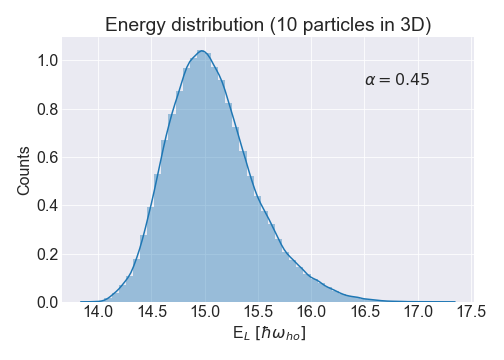
\includegraphics[width=0.5\linewidth]{../Results/histogram_10p_3d_alpha_45}\caption{A histrogram of the local energy distribution for the calculation where $\alpha = 0.45$ in Tab. \ref{tab:brute_force_N_10}.}\label{fig:histogram}
\end{figure}

The resulting energies and standard deviations for calcualtions of the system with higher number of particles (50 particles, 100 particles and 500 particles) can be found in Appendix \ref{app:alpha_lists_brute_force}. Those calculations show a similar behavoir and were therefore not included here. 

\subsection{Including importance sampling}

Figure \ref{fig:compare_importance_steps} shows that with brute force sampling there seems to be a trade-off between the acceptance and the accuracy of the result. The right plot shows that larger steps, to a certain point, will give a better accuracy, but, as can be observed in plot to the left, the acceptance decreases with larger step lengths, $dl$. We also see that for smaller step sizes, the brute force sampling's accuracy is very poor, at least for $2^{20}$ number of MC cycles. From the comparison of the two plots a  step length at $dl = 0.5 = 5\cdot10^{-1}$ seems to give the best trade-off when using brute force sampling with $2^{20}$ number of MC cycles.

With importance sampling, on the other hand, both acceptance and accuracy increases with smaller time steps ($\Delta t$). A time step at $\Delta t = 0.005 = 5\cdot10^{-3}$ seems to be a good choice with $2^{20}$ number of MC cycles according to Fig. \ref{fig:compare_importance_steps}. 

\begin{figure}[H]
\center
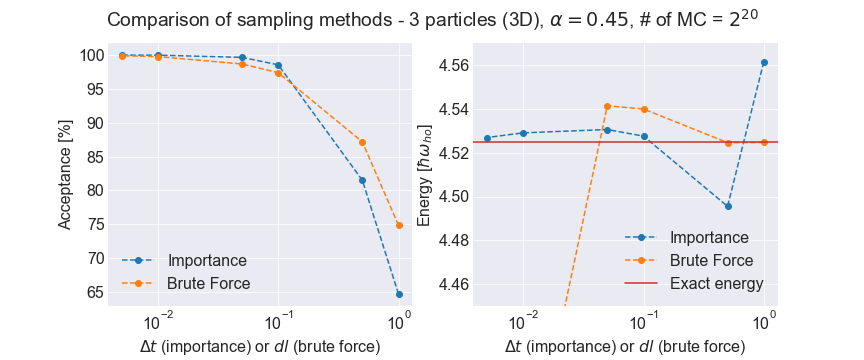
\includegraphics[width=\linewidth]{../Results/comparison_steps_importance}\caption{A comparison between brute force sampling and importance sampling. Left: The acceptance percent of suggested moved as a function of step length ($dl$) or time step ($\Delta t$). Right: The expectation value of the energy after $2^{20}$ steps and $\alpha = 0.45$ compared with the exact energy $\alpha = 0.45$. }\label{fig:compare_importance_steps}
\end{figure}

Figure \ref{fig:compare_importance_MC} was made using the step sizes extracted from Fig. \ref{fig:compare_importance_steps}. The figure shows that both sampling methods give accurate values (within $\pm$ 0.004 of the exact value) for number of MC cylces above $2^{20}$, at least for three particels in three dimensions.

\begin{figure}[H]\caption{A comparison of the behavoir of the different sampling methods with regards to number of MC cycles.}\label{fig:compare_importance_MC}
\center
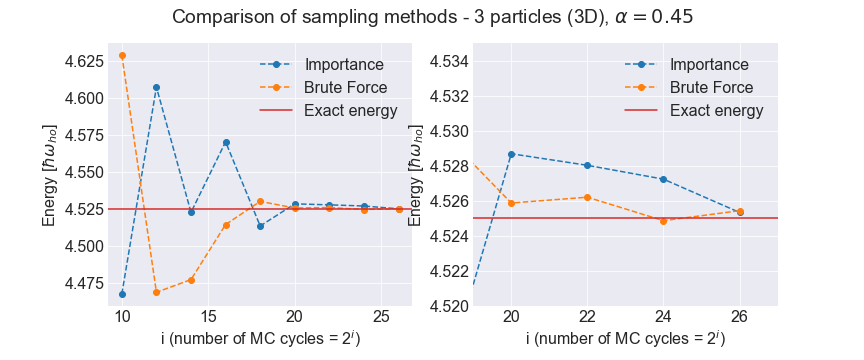
\includegraphics[width=\linewidth]{../Results/comparison_MC_importance}
\end{figure}

Table \ref{tab:importance_N_1} and Tab. \ref{tab:importance_N_10} shows the resulting energies and standard deviations from calculations with importance sampling for one and ten particles in three dimensions respectively. The numbers are very similar to the calcualted values from the brute force sampling method, but this is expected from the results in Fig. \ref{fig:compare_importance_steps} and Fig. \ref{fig:compare_importance_MC} which show that the expectation energies from the two methods are similar with number of MC cycles above $2^{20}$ and an appropriate $dl$ or $\Delta t$. 

\textit{Should probably compare the expectation values like in Fig. \ref{fig:equilibrium}?}

\begin{table}[H]\caption{The calculated energies, $\left<E_L\right>$, for one particle in three dimensions compared with the exact energy, $E_{ex}$. Both energies are of units $\hbar\omega_{oh}$. These calculations were performed with $2^{20}$ number of MC cycles. The normal standard deviation $\sigma$, and the variance from the blocking resampling method, $\sigma_B$ are also included. }\label{tab:importance_N_1}
\center
\begin{tabular}{cccccc}
$\alpha$ & $\left< E_L \right>$ & $E_{ex}$ & |$\left< E_L \right>-E_{ex}$|  & $\sigma_B$ & $\sigma$\\ \hline
0.35 & 1.59139 & 1.59643 & 0.00504 & 0.00965 & 0.43954\\
0.40 & 1.53229 & 1.53750 & 0.00521 & 0.00550 & 0.27462\\
0.45 & 1.50692 & 1.50833 & 0.00141 & 0.00243 & 0.12940\\
0.50 & 1.50000 & 1.50000 &                &                &                 \\
0.55 & 1.50696 & 1.50682 & 0.00014 & 0.00201 & 0.11744\\
0.60 & 1.52597 & 1.52500 & 0.00097 & 0.00343 & 0.22232\\
0.65 & 1.55742 & 1.55192 & 0.00549 & 0.00509 & 0.32402\\
\end{tabular}
\end{table} 

\begin{table}[H]\caption{The calculated energies, $\left<E_L\right>$, for ten particle in three dimensions compared with the exact energy, $E_{ex}$. Both energies are of units $\hbar\omega_{oh}$. These calculations were performed with $2^{20}$ number of MC cycles. The normal standard deviation, $\sigma$, and the standard deviation from the blocking resampling method, $\sigma_B$ are also included.}\label{tab:importance_N_10}
\center
\begin{tabular}{cccccc}
$\alpha$ & $\left< E_L \right>$ & $E_{ex}$ & |$\left< E_L \right>-E_{ex}$|  & $\sigma_B$ & $\sigma$\\ \hline
0.35 & 15.98097 & 15.96429 & 0.01668 & 0.09399 & 1.47776\\
0.40 & 15.33029 & 15.37500 & 0.04471 & 0.04686 & 0.85013\\
0.45 & 15.07401 & 15.08333 & 0.00932 & 0.02182 & 0.38900\\
0.50 & 15.00000 & 15.00000 &                &                &                \\
0.55 & 15.07112 & 15.06818 & 0.00294 & 0.01612 & 0.36242\\
0.60 & 15.19266 & 15.25000 & 0.05734 & 0.03098 & 0.70746\\
0.65 & 15.54807 & 15.51923 & 0.02884 & 0.04239 & 0.98210\\
\end{tabular}
\end{table} 

\subsection{Including optimization with simple  gradient descent methods}

We will now look at optimization and spesifically the simple gradient descent methods described in section \ref{sec:gradient} and \ref{sec:gradient2}. Figure \ref{fig:gradient_descent_starts} shows how the efficiency of the simple gradient descent method is dependant on the first guess, the start value of $\alpha$. We observe that, naturally, the algorithm is faster when the guess is closer to the exact parameter ($\alpha = 0.5$). 

\begin{figure}[H]\caption{A comparison of different start values for the parameter $\alpha$. The algorithm stops when the energy difference is less then $1\cdot10^{-5}$ from one step to the next. The diamond shape marker is added to emphasis at what step this critera is fulfilled. Left: The development of $\alpha$. Right: the development of the expectation value.}\label{fig:gradient_descent_starts}
\center
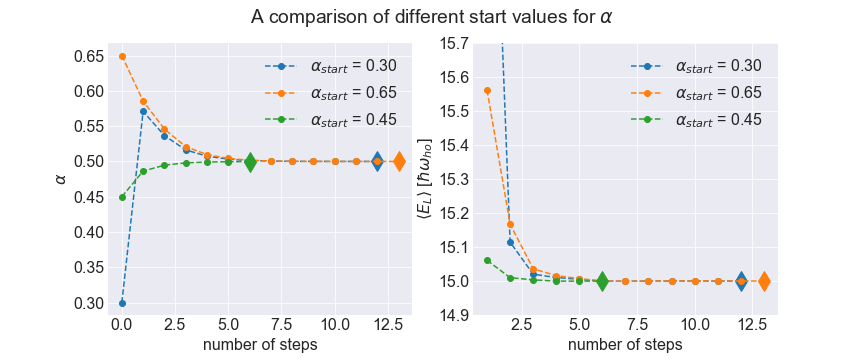
\includegraphics[width=\linewidth]{../Results/gradient_descent_starts}
\end{figure}

Figure \ref{fig:gradient_descent_rates} shows that the minimization rate, $\lambda$, cannot be too small, then the algorithm moves very slowly toward the minimum as observed for $\lambda = 0.01$. On the other hand, if the rate is too big it also moves slowly toward the $\alpha$ that gives the minimum, but ocsillating between values larger and smaller than the $\alpha$ that gives the minimum energy. From the figure we observe that $\lambda$ is the most effecive minimization rate.

\begin{figure}[H]\caption{A comparison of different minimization rates using the simple gradient descent method from section \ref{sec:gradient}. Here $\lambda$ is the minimization rate. The diamond markers are used to show at which step the difference between the last two energies were less than $1\cdot 10^{-5}$.} \label{fig:gradient_descent_rates}
\center
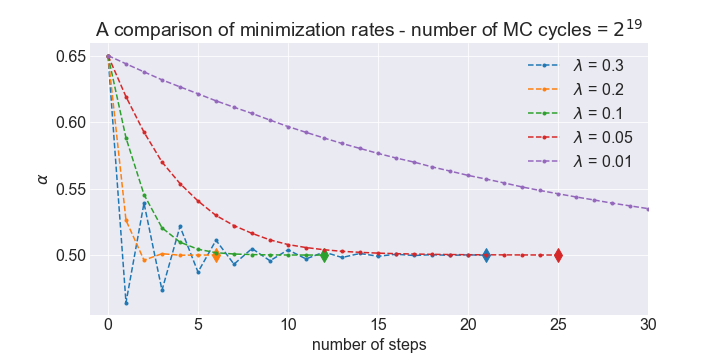
\includegraphics[width=0.8\linewidth]{../Results/gradient_minimization_rate}
\end{figure}

Figure \ref{fig:gradient_descent_lambda} shows how the simple gradient descent method can be made more efficient by including the gradient calculated for the previous step. Similarly to the evaluation of $\gamma$, a $\lambda$ that is not too small (will result in the same result as for the simple gradient descent method) and not too large has to be found. Here we observe that $\lambda = 0.02$ is the best choice when $\gamma = 0.1$. Even though this more complex gradient method can make the simple gradient method more effective the difference is not crusial for this project and the simple gradient descent method is good enough.

\begin{figure}[H]\caption{A comparison of the two gradient descent methods described in section \ref{sec:gradient} and \ref{sec:gradient2}. The algorithm stops when the energy difference is less then $10^{-5}$ from one step to the next. Here $\lambda$ is the weigth of the previous gradient's influence on the next pick of $\alpha$. The inset plot shows how many steps is needed to reach this critera the different $\lambda$s. The dotted blue line shows the number of steps needed for the simple gradient descent method.}\label{fig:gradient_descent_lambda}
\center
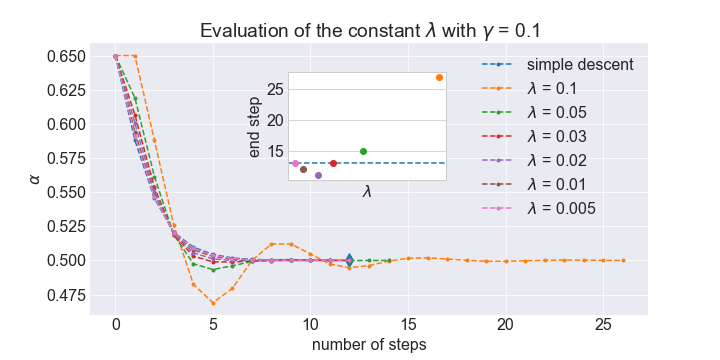
\includegraphics[width=0.8\linewidth]{../Results/comparing_gradient_descents.png}
\end{figure}



\subsection{Including interaction and an elliptical trap}

Here we have added an interaction potential in the hamiltonian and hence included an interaction term in the wavefunction. This is all described in the teory part of this report and how it is implemented in the code to calculate the local energy and the drift force is described in Appendix \ref{sec:implementation}.

\begin{table}[H]\caption{The calculated energies, $\left<E_L\right>$, for ten particle in three dimensions compared with the exact energy for the non-interacting case, $E_{ex}$. Both energies are of units $\hbar\omega_{oh}$. These calculations were performed with $2^{20}$ number of MC cycles. The normal standard deviation, $\sigma$, and the standard deviation from the blocking resampling method, $\sigma_B$ are also included.}\label{tab:interaction_N_10}
\center
\begin{tabular}{cccccc}
$\alpha$ & $\left< E_L \right>$ & $E_{ex}$(no int.) & |$\left< E_L \right>-E_{ex}$|  & $\sigma_B$ & $\sigma$\\ \hline
0.35 & 16.16895 & 15.96429 & 0.20466 & 0.04723 & 1.39931\\
0.40 & 15.57277 & 15.37500 & 0.19777 & 0.02440 & 0.82444\\
0.45 & 15.33414 & 15.08333 & 0.25080 & 0.01153 & 0.37842\\
0.50 & 15.25790 & 15.00000 & 0.25790 & 0.00120 & 0.07902\\
0.55 & 15.35359 & 15.06818 & 0.28541 & 0.01228 & 0.41498\\
0.60 & 15.58890 & 15.25000 & 0.33890 & 0.01847 & 0.74266\\
0.65 & 15.84713 & 15.51923 & 0.32789 & 0.02895 & 1.09169\\
\end{tabular}
\end{table} 

% \begin{equation}
% E_L = -\frac{\hbar^2}{2m} \sum_k^N \left( \frac{\partial^2}{\partial x_k^2} \phi(x_k,y_k,z_k)  + \frac{\partial^2}{\partial y_k^2} \phi(x_k,y_k,z_k) + \frac{\partial^2}{\partial z_k^2} \phi(x_k,y_k,z_k) \right) + \frac{1}{2}m \omega^2 \sum_k^N \left( x_k^2 + y_k^2 +z_k^2 \right)
% \end{equation}